\documentclass[10pt]{article}
\usepackage[a4paper, total={6in, 10in}]{geometry}
\usepackage{blindtext}
\usepackage[colorlinks,allcolors=blue]{hyperref}
\usepackage{titling}
\usepackage{authblk}
\usepackage{graphicx}
\usepackage{listings}
\usepackage{xcolor}

\graphicspath{ {./img/} }

\colorlet{punct}{red!60!black}
\definecolor{delim}{RGB}{20,105,176}
\colorlet{numb}{magenta!60!black}
\lstdefinelanguage{json}{
    basicstyle=\normalfont\ttfamily,
    numbersep=8pt,
    showstringspaces=false,
    breaklines=true,
    literate=
     *{0}{{{\color{numb}0}}}{1}
      {1}{{{\color{numb}1}}}{1}
      {2}{{{\color{numb}2}}}{1}
      {3}{{{\color{numb}3}}}{1}
      {4}{{{\color{numb}4}}}{1}
      {5}{{{\color{numb}5}}}{1}
      {6}{{{\color{numb}6}}}{1}
      {7}{{{\color{numb}7}}}{1}
      {8}{{{\color{numb}8}}}{1}
      {9}{{{\color{numb}9}}}{1}
      {:}{{{\color{punct}{:}}}}{1}
      {,}{{{\color{punct}{,}}}}{1}
      {\{}{{{\color{delim}{\{}}}}{1}
      {\}}{{{\color{delim}{\}}}}}{1}
      {[}{{{\color{delim}{[}}}}{1}
      {]}{{{\color{delim}{]}}}}{1},
}

\predate{}
\postdate{}

\title{Accelerating Research with AWS IoT}
\author[1]{Marcilio Mendonca}
\author[1]{Bruno Vitali}
\author[1]{Arjun Shakdher}
\author[2]{Brent Maranzano}
\author[2]{Giuseppe Cogoni}
\author[2]{Bo Du}
\author[1]{Bryan Stone}
\author[1]{Don Bennett}

\affil[1]{AWS}
\affil[2]{Pfizer, Inc.}

\date{} % clear date
\begin{document}

\maketitle


\section*{}

The speed of designing synthetic routes and defining 
formulations for new drug substances can be limited by the
rate at which the data becomes available for decision making. 
Much of the data is generated by offline laboratory
experiments, which requires process sampling, subdividing, 
transporting and consequently time-consuming sample 
preparation prior to analysis, in addition to the time
to analyze, interpret and report the results. An obvious
path to accelerate sample measurements is to increase the
number of analyses that can be performed in parallel by
either increasing the staff or through automation.
Alternatively, the entire process can be shortened by performing
the analysis in-situ. This approach, referred to as 
Process Analytical Technology (PAT), has been used in the
pharmaceutical industry for decades, but has been limited
to monitoring a few key parameters, most commonly using spectroscopic tools. 
The advent of miniature, cheap electronics coupled 
with the Internet of Things (IoT) has opened the possibility of 
monitoring a wide range of parameters in real-time.

\section*{Motivations}

The one obstacle that has inhibited the widespread adoption
of IoT in the pharmaceutical industry is the lack of a secure, 
scalable and cost-effective platform that can be used to store, 
analyze and visualize the data. 

In this post, it is described the development of a
combination of on-premise and cloud-based IoT platform
that can be used to monitor and analyze data from a wide
range of sensors. This was achieved through the Pfizer's SmartLab initiative
and in collaboration with AWS to integrate its IoT services.


\section*{Architecture}
The key to a successful IoT platform is the ability to
scale to a large number of devices that can be readily implemented 
in various processes with minimal experience or training
by the end user e.g.: “plug-n-play”. 
This minimal training interface often requires developing custom
in-house applications that make calibration, measurement
and analysis simple and robust. Moreover, the IoT platform 
must handle the large amount of data generated by
the sensors securely and cost-effectively. One way to achieve this 
goal is through the use of AWS IoT services and solutions, which allow to
connect, collect, store and analyze IoT data for industrial workloads.

At Pfizer, for this PoC, the PAT sensors communicate to the AWS IoT Core broker
through a Mosquitto MQTT broker/bridge that communicates from 
the Pfizer lab network to a Rapid Virtual Private Cloud (VPC) sub-network. 
A web dashboard was also developed to be able to visualize and control 
each instrument that connects to a public AWS VPC and through a transit 
gateway, to the Rapid VPC for the data exchange. A schematic, summarizing 
this hybrid on-premise/cloud architecture is shown on Figure \ref{architecture}.

\begin{figure}[h]
\centering
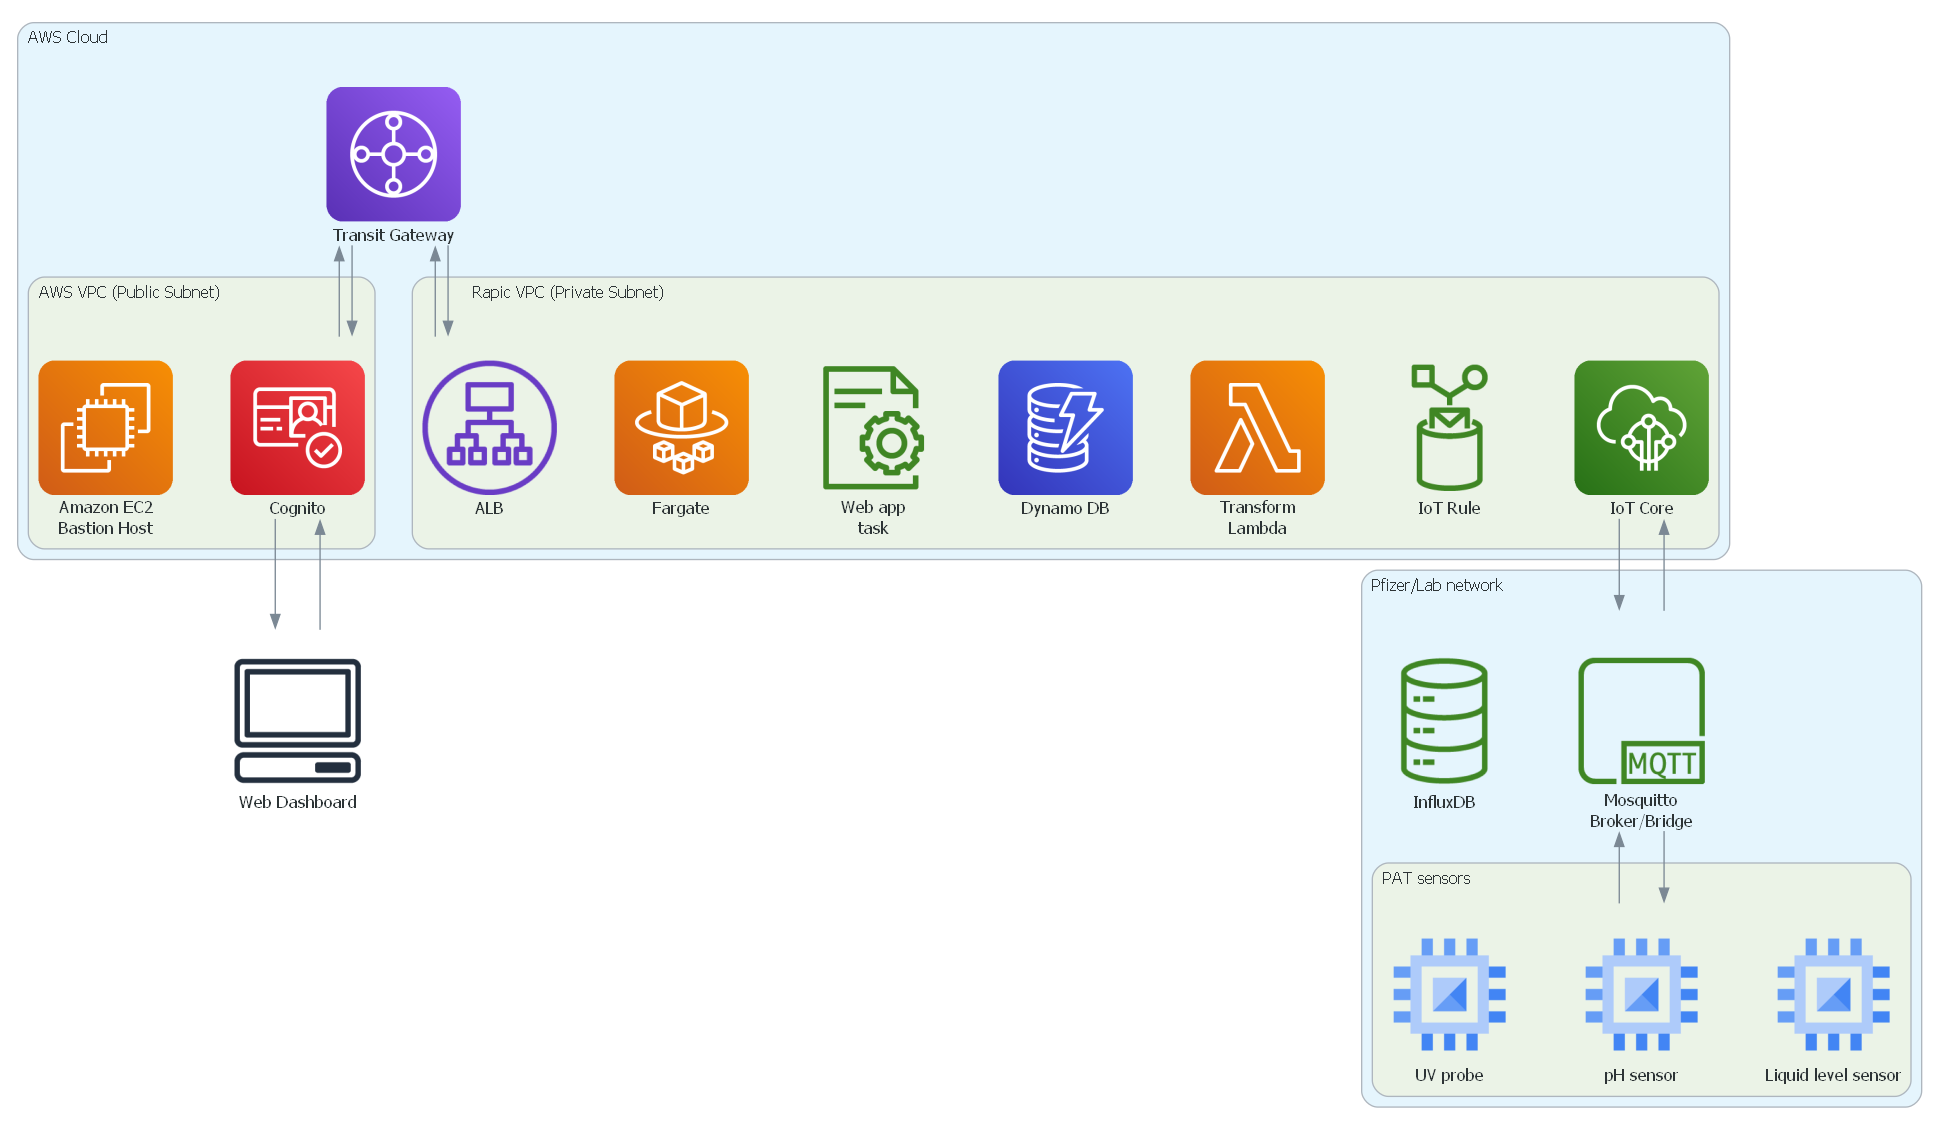
\includegraphics[width=1\textwidth]{architecture}
\caption{Pfizer/AWS IoT architecture.}
\label{architecture}
\end{figure}


\section*{Interfacing the laboratory instruments}
For this PoC, three commonly used PAT sensors were utilized in order
to cover different data types that can be exchanged, these include:
\begin{enumerate}
	\item A level sensor, for process safety applications
	(generating Boolean data type);
	\item A pH sensor (generating scalar data type);
	\item An UV spectrometer (generating array data type).
\end{enumerate}
Each of instrument is connected to a hardware wrapper
(Raspberry Pi\texttrademark\ or ESP32 microcontroller)
that aims to convert and exchange the control commands and data from 
its native protocol into a standard-based messaging protocol, MQTT, following
the payload structure according to the Eclipse Foundation
\href{https://sparkplug.eclipse.org/specification/version/2.2/documents/sparkplug-specification-2.2.pdf}{Sparkplug\texttrademark} B specification. An example of data payload 
(DDATA) coming from one of the instrument is showed in Figure \ref{spark}.

\begin{figure}[h]
\centering
\begin{tabular}{c}
\begin{lstlisting}[language=json,
				   basicstyle=\small]
{
  "timestamp": "1701199950000",
  "seq": 14,
  "metrics": [
    {
      "name": "status",
      "timestamp": "1701199950000",
      "dataType": "Uint32",
      "value": 0
    },
    {
      "name": "level_high",
      "timestamp": "1701199950000",
      "dataType": "Uint32",
      "value": 0
    }
  ]
}
\end{lstlisting}
\end{tabular}
\caption{Example of MQTT payload following Sparkplug\texttrademark B.}
\label{spark}
\end{figure}

The local communication within the lab network is then managed through 
an Eclipse Mosquitto\texttrademark\ MQTT broker, configured to bridge and 
share the communication with the AWS cloud managed MQTT broker, 
\href{https://aws.amazon.com/iot-core/?nc=sn&loc=0}{IoT Core} service, 
residing within a Rapid VPC, as a private sub-network.


\section*{Data storage visualization and instrument control}

The data generated by each instrument is locally stored within the Pfizer lab
network into an Influx database as well as within the AWS cloud,
into a Dynamo DB, this last is then utilized as the data source for
the web dashboard, used as instrument control platform and data visualization.
The web dashboard interfaces to the Rapid VPC, through a transit gateway,
that communicated to the public AWS VPC where it uses the Cognito service of
AWS for user authentication.

\begin{figure}[h]
\centering
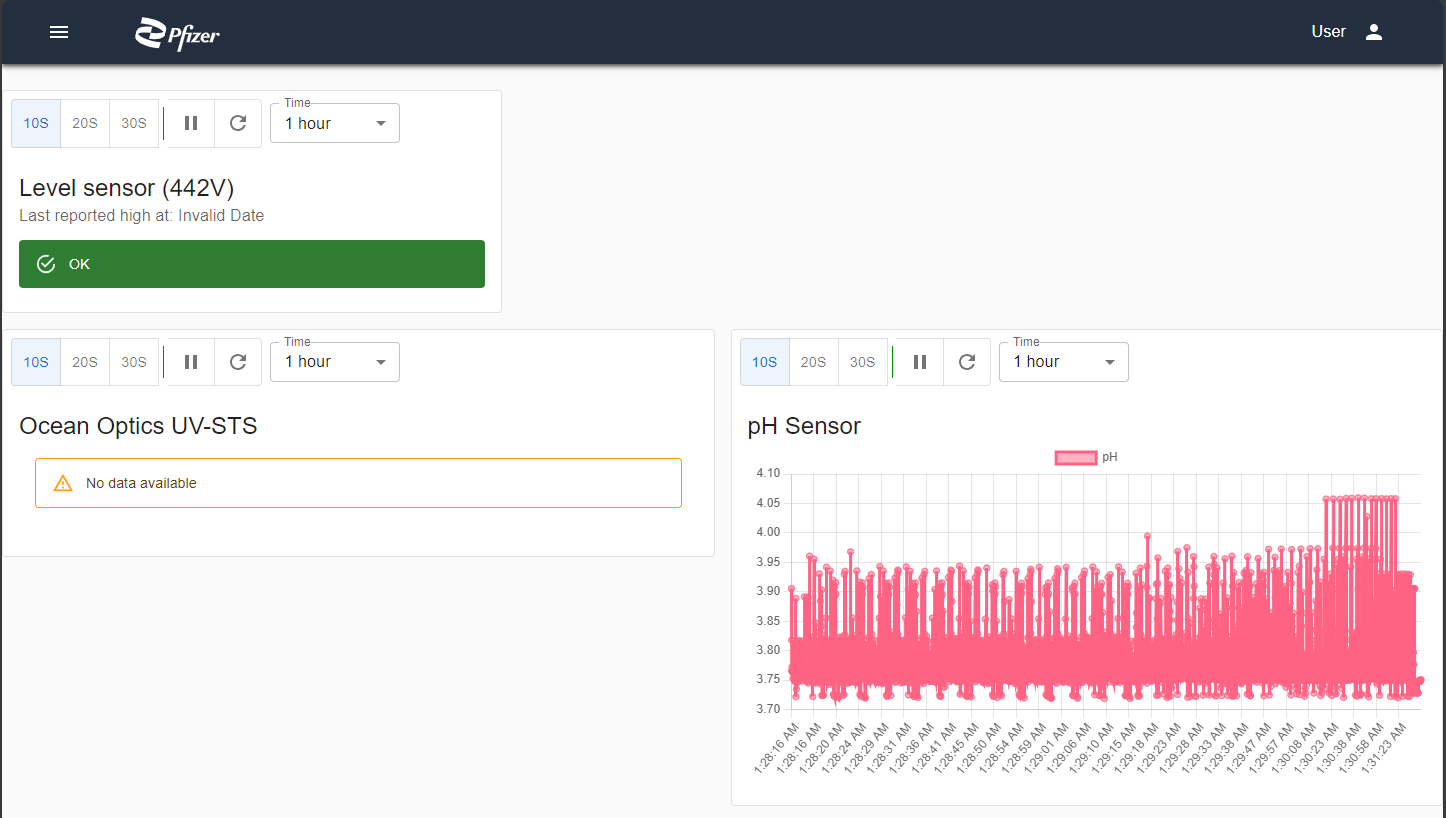
\includegraphics[width=1\textwidth]{webapp_aws}
\caption{Data visualization web app dashboard.}
\label{webapp_aws}
\end{figure}

\begin{figure}[h]
\centering
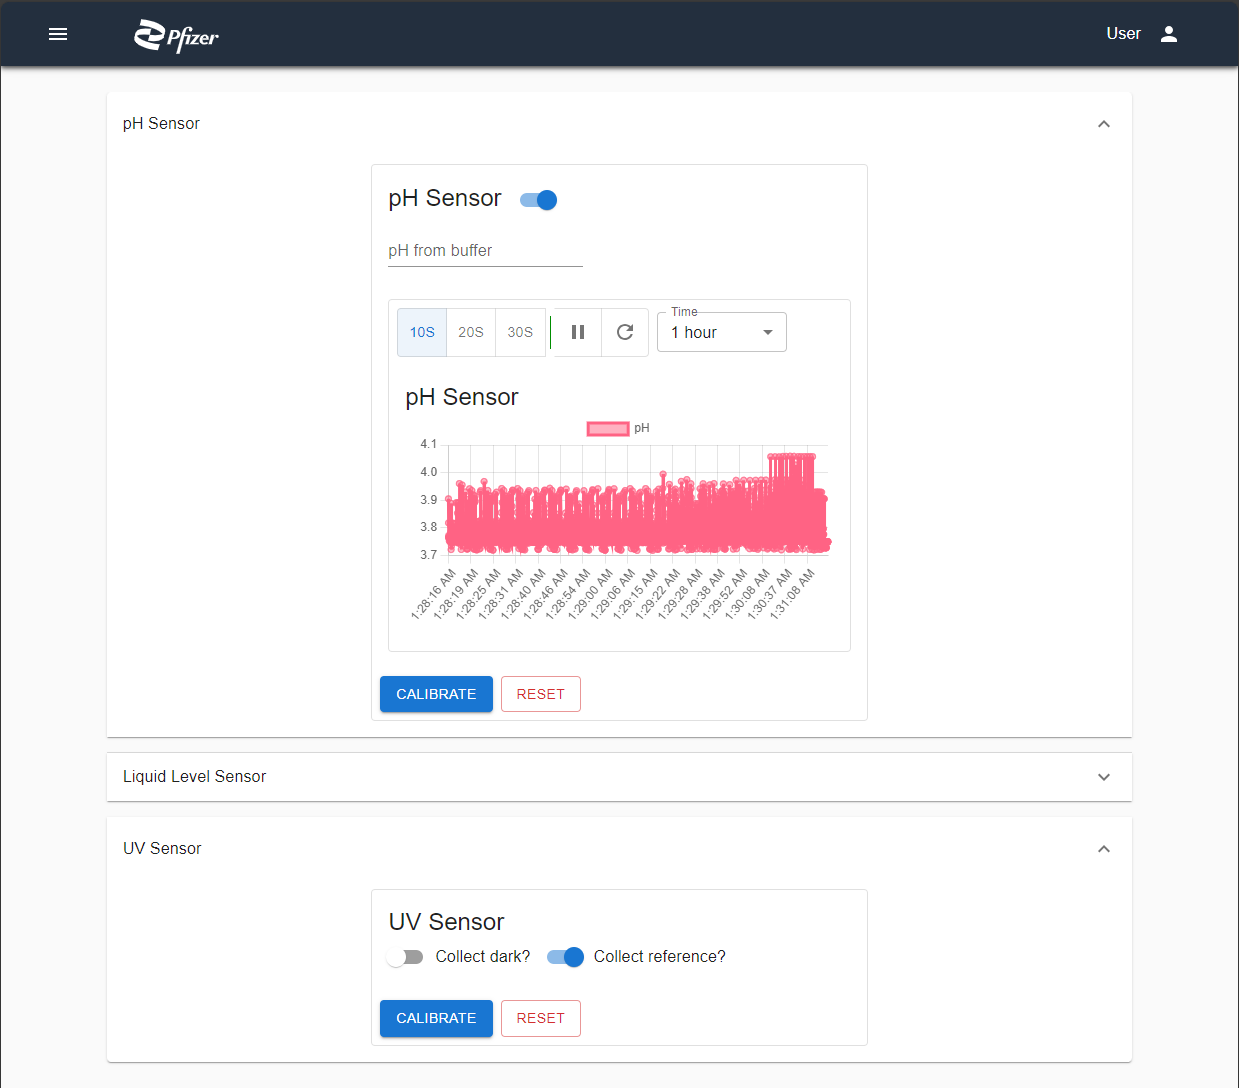
\includegraphics[width=1\textwidth]{webapp_aws2}
\caption{Instrument calibration panel withing webapp.}
\label{webapp_aws2}
\end{figure}

Once connected, the user has the option to visualize the data
(Figure \ref{webapp_aws}) and/or calibrate the instrument(s)
(Figure \ref{webapp_aws2}). The instrument calibration was part of the PoC
to test the bidirectionality of the communication and the ability to
remotely control the individual instruments.

\section*{Conclusions}

In this blog post, we have described how Pfizer through its SmartLab initiative,
alongside Amazon AWS was able to implement and deploy a secure, 
scalable and cost-effective platform that can be used to store, 
analyze and visualize the data coming from PAT instruments.

With the discussed PoC it will be possible to modularize the deployment
to multiple lab areas, also across multiple sites and be able to access to the data
and control each individual instrument virtually from anywhere within the company.

\end{document}